\chapter{Background and Fundamental Aspects}
\label{chap:ch2}
\hspace{\parindent}
This chapter presents the fundamental concepts and background knowledge required to contextualize
the research developed in this dissertation. Section~\ref{sec:problem-definition} introduces the
MRPP problem considered in this work and explains how it can be formalized through the MAPF
abstraction. Section~\ref{sec:mapf-representation} discusses the environment representations used
to instantiate this type of planning problem. Section~\ref{sec:single-agent-search} explores
classical graph search algorithms that serve as building blocks for many MRPP methods.
Section~\ref{sec:ml_foundations} introduces machine learning concepts used to support the
heuristic analysis. Finally, Section~\ref{sec:parallel-concurrent} presents foundational notions of
parallel and concurrent computing.

\section{MAPF Problem: Formal Definition }
\label{sec:problem-definition}

\paragraph{}
The MAPF problem concerns the computation of collision-free trajectories for a group of cooperative agents that must move from their initial states to their target states while operating in a shared environment. Each agent must reach its goal without colliding with other agents, while a global performance criterion is optimized. This general problem formulation follows the, widely adopted, conceptual definition of MAPF presented by Stern et al.~\cite{stern2019definitions}. While that work instantiates the problem on graph-based environments, the underlying definition is independent of the specific representation and can be abstracted to more general state spaces.

From a formal perspective, let there be a set of $m$ agents $A = \{a_1, a_2, \dots, a_m\}$. Each agent $a_i \in A$ is associated with an initial state $s_i$ and a goal state $g_i$.


A solution for an agent $a_i$ is defined as a trajectory $P_i$, which specifies the evolution of the agent’s state over time. In discrete formulations, a trajectory can be represented as a sequence of states
\begin{equation}
P_i = \langle p_i^0, p_i^1, \dots, p_i^T \rangle
\end{equation}
where $p_i^0 = s_i$ and $p_i^T = g_i$. 
The explicit consideration of time is essential in MAPF, as interactions and conflicts between agents arise from the simultaneous execution of their trajectories in a shared space-time domain \cite{stern2019definitions}.

A valid MAPF solution must ensure that no two agents are in conflict during their motion, where conflicts arise when agents attempt to occupy incompatible states in space and time.
 The most common type of conflict is the position conflict, which occurs when two agents occupy the same state at the same time step, i.e., $p_i^t = p_j^t$ for $i \neq j$. Other types of conflicts may arise depending on the motion model and representation adopted, but all correspond to violations of mutual feasibility constraints among agents \cite{stern2019definitions}.

The objective of MAPF is to compute a set of conflict-free trajectories $\{P_1, P_2, \dots, P_m\}$ that minimize a global cost function $C$. This cost function is defined over the joint set of agent trajectories and encodes the chosen optimization criterion. Common objectives include minimizing the time at which the last agent reaches its goal (makespan) or minimizing the sum of individual agents’ traversal costs, as commonly considered in the literature. Formally:

\begin{tcolorbox}[colback=gray!5!white, colframe=gray!30, boxrule=0.3pt, arc=3pt, left=3pt, right=3pt, top=1pt, bottom=1pt]
\vspace{-3pt}
\[
\textbf{Find } \{P_1, P_2, \dots, P_m\} \textbf{ such that} \text{ all trajectories are conflict-free and } C(\{P_i\}) \text{ is minimized.}
\]
\vspace{-6pt}
\end{tcolorbox}

The MAPF problem is combinatorial in nature and is NP-hard in the general case, as formally established in earlier works \cite{surynek2010, yu2013planning} and confirmed in recent complexity analyses \cite{geft2022refined, gao2024review}. This inherent complexity motivates the development of planning algorithms that aim to balance solution quality with computational efficiency.


\section{Environment Representation}
\label{sec:mapf-representation}
\hspace{\parindent}
Although MRPP can be described independently of a specific environment representation, practical
planning methods require a concrete state space in which robot motion and conflicts can be
evaluated. In multi-robot planning literature, different representations have been adopted,
primarily differing in how space and time are modeled and in the resulting level of abstraction.

Common approaches include discrete representations, such as grids and graphs, where robots occupy
a finite set of states and move between neighboring states in discrete time steps, as well as
continuous formulations, where robot motion is described by continuous trajectories and conflicts
arise from geometric interactions. Figure~\ref{fig:env_representations} illustrates how the same
workspace can be modeled under different discrete representations.

While continuous formulations offer higher modeling fidelity, discrete representations are widely
used in classical MAPF and MRPP settings due to their simplicity and structured abstraction. In this
dissertation, the focus is placed on grid and graph representations, with particular emphasis on
graph representations because the considered fleet coordination framework performs planning over a
shared roadmap.

\begin{figure}[H]
    \centering
    \begin{subfigure}{0.30\linewidth}
        \centering
        
\includegraphics[width=\linewidth]{original_ground.png}
        \caption{Workspace layout}
    \end{subfigure}
    \hspace{0.5em}
    \begin{subfigure}{0.30\linewidth}
        \centering
        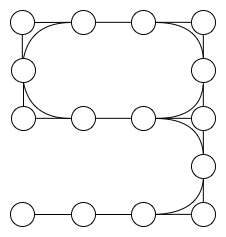
\includegraphics[width=\linewidth]{graph.png}
        \caption{Graph representation}
    \end{subfigure}
    \hspace{0.5em}
    \begin{subfigure}{0.30\linewidth}
        \centering
        
\includegraphics[width=\linewidth]{grid.png}
        \caption{Grid representation}
    \end{subfigure}

    \caption{Illustration of different discrete environment representations for the same workspace.}
    \label{fig:env_representations}
\end{figure}


\subsection{Grid Representation}
\label{subsec:grid_representation}
\hspace{\parindent}
In grid formulations, the environment is discretized into a regular two or three-dimensional array
of uniformly sized cells, each classified as free or occupied. Robots move between neighboring
cells according to a fixed connectivity structure, yielding a simple and intuitive abstraction that
has been widely adopted in early MAPF studies
\cite{yang2010grid,stern2019definitions}.

A key advantage of grid representations is their simplicity and direct correspondence to occupancy
grids used in robotic perception. However, grid resolution introduces an inherent trade-off. Coarse
grids may fail to capture narrow passages or thin obstacles, while fine grids incur substantial memory
and computational costs \cite{yang2010grid,ma2022graph}. In addition, the discrete nature of grid
motion complicates the integration of continuous-time dynamics, often requiring post-processing to
obtain executable trajectories \cite{ma2022graph}.

For these reasons, graph representations are particularly relevant in this dissertation, since the
considered fleet coordination framework performs planning over a shared roadmap~\cite{matos2025criis}. By allowing
arbitrary topologies and connectivity patterns, graph representations provide a convenient
abstraction for modeling structured environments and for supporting centralized coordination.


\subsection{Graph Representation}
\hspace{\parindent}
In graph formulations the environment is modeled as a discrete graph that
captures admissible robot states and their connectivity. This follows the modeling approach
described by Stern et al.~\cite{stern2019definitions}, while being interpreted here in the context of
multi-robot fleet coordination.

Formally, the environment is represented as a graph \(G = (V, E)\), where each vertex
\(v \in V\) corresponds to a valid state that a robot may occupy, and each edge \((u,v) \in E\)
encodes a feasible transition between states. The graph may be directed or undirected, depending on
the characteristics of the environment and on the motion constraints imposed by the planning system.

Under this representation, robot trajectories evolve in discrete time steps and are constrained to
lie on the graph. Each state \(p_i^t\) therefore corresponds to a vertex in \(V\), and successive
states satisfy
\[
p_i^{t+1} = p_i^t
\quad \text{or} \quad
(p_i^t, p_i^{t+1}) \in E.
\]
The first case represents a waiting action, while the second represents a
movement between two connected vertices~\cite{yu2013planning}.


\subsubsection{Graph Construction Approaches}
\hspace{\parindent}
Several classical approaches have been proposed to construct graph representations of planning
environments. These include roadmap approaches such as visibility graphs, which connect mutually
visible obstacle vertices \cite{lozano1979algorithm}, Voronoi diagram representations that
emphasize obstacle clearance \cite{aurenhammer1991voronoi}, and cell decomposition techniques that
subdivide the free space into regions whose adjacency defines a connectivity graph
\cite{latombe1991robot,choset2005principles}. Representative examples of these constructions are
illustrated in Figure~\ref{fig:classical_graph_construction}.

In this dissertation, the objective is not to compare graph construction methods, but to perform
multi-robot coordination over an existing graph representation. The underlying roadmap is therefore
assumed to be available, and the planning problem consists of computing coordinated robot
trajectories on top of this discrete abstraction.

\begin{figure}[H]
    \centering
    \begin{subfigure}{0.35\linewidth}
        \centering
        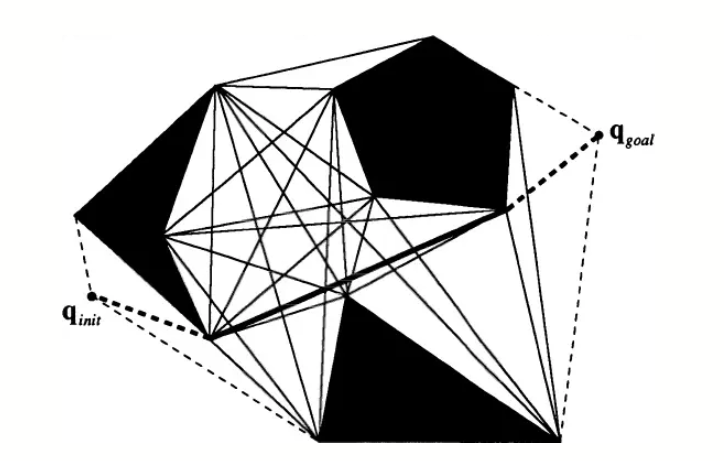
\includegraphics[width=\linewidth]{visibility_graph.png}
        \caption{Visibility graph}
    \end{subfigure}
    \hfill
    \begin{subfigure}{0.27\linewidth}
        \centering
        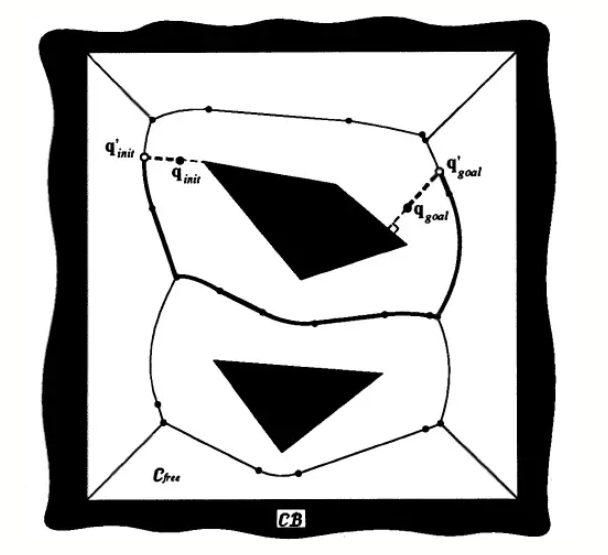
\includegraphics[width=\linewidth]{voronoi.png}
        \caption{Voronoi diagram}
    \end{subfigure}
    \hfill
    \begin{subfigure}{0.32\linewidth}
        \centering
        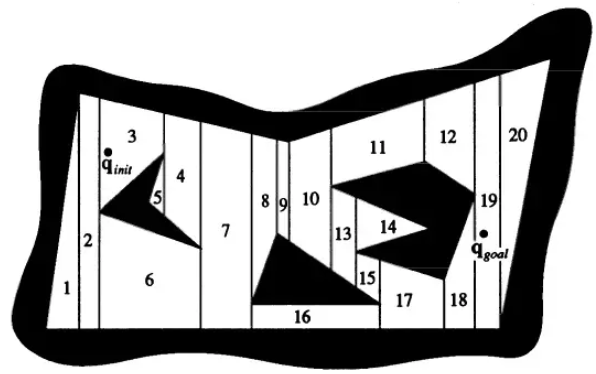
\includegraphics[width=\linewidth]{cell_decomposition.png}
        \caption{Cell decomposition}
    \end{subfigure}
    \caption{Classical approaches for constructing graph representations \cite{latombe1991robot}.}
    \label{fig:classical_graph_construction}
\end{figure}


\section{Search and Planning Foundations}
\label{sec:single-agent-search}
\hspace{\parindent}
Classical graph search techniques provide an important foundation for MRPP and MAPF methods,
since they are commonly used to compute individual robot paths and to support coordination
strategies. In the context of this dissertation, these methods are particularly relevant because the
considered fleet coordination framework performs planning over a graph representation of the
environment.

Accordingly, this section reviews graph search and planning concepts that underlie the TEA*
planner used in this work and many related multi-robot coordination approaches. The focus is first
placed on shortest path search in graphs and then on heuristic search, with particular emphasis on
Dijkstra's algorithm and A*.



\subsection{Search Problems on Graphs}
\hspace{\parindent}
A search problem on a graph consists of finding a sequence of transitions that leads from a
given initial state to a goal state while satisfying feasibility constraints and optimizing a
specified cost criterion \cite{russell2010aima}.

Formally, a search problem is defined by a state space, an initial state, a set of goal states,
a transition model that specifies the allowable moves between states, and a cost function that
assigns a non-negative cost to each transition or path \cite{russell2010aima}. When the state
space is represented explicitly as a graph, vertices correspond to states and edges encode
feasible transitions, possibly associated with traversal costs.

A solution to a graph search problem is a path in the graph that connects the initial vertex
to a goal vertex. Among all feasible solutions, particular interest is often placed on optimal
solutions, defined as those that minimize the cumulative cost along the path. The shortest path
problem in weighted graphs is a canonical instance of this formulation and has been extensively
studied in both theoretical and applied contexts \cite{cormen2009introduction}.

Search algorithms typically operate by incrementally exploring the graph starting from the
initial state, expanding states according to a specific strategy and maintaining a frontier of
candidate paths. Different search strategies define different orders in which states are
expanded, which directly affects properties such as completeness, optimality, and computational
efficiency \cite{hart1968formal}.

\subsubsection{Dijkstra's Algorithm}
\hspace{\parindent}
Dijkstra's algorithm is a classical graph search algorithm for solving the shortest path problem
in weighted graphs with non-negative edge costs. Originally introduced by Dijkstra
\cite{dijkstra1959note}, it provides a systematic procedure for computing the minimum-cost path
from a given initial vertex to all other reachable vertices in the graph.

The algorithm operates by incrementally expanding vertices in order of increasing accumulated
path cost from the initial state. At each step, the vertex with the lowest known cost is selected
for expansion, and its outgoing edges are relaxed to update the cost of reaching neighboring
vertices. This process continues until the goal vertex is reached or all reachable vertices have
been explored \cite{cormen2009introduction}.
A key property of Dijkstra's algorithm is that, under the assumption of non-negative edge costs,
once a vertex is expanded, the cost associated with it is guaranteed to be optimal. As a result,
the algorithm is both complete and optimal for this class of graphs \cite{cormen2009introduction}.

From a search perspective, Dijkstra's algorithm can be viewed as a best-first search strategy in
which the expansion order is determined by the accumulated path cost from the initial
vertex. This accumulated cost, commonly denoted by $g(n)$ for a vertex $n$, corresponds to the
sum of the costs of the edges along the path from the initial vertex to $n$
\begin{equation}
\label{eq:gn}
g(n) = \sum_{(u,v) \in P_n} c(u,v),
\end{equation}
where $P_n$ denotes the path to $n$ and $c(u,v)$ is the cost of edge from vertex $u$ to vertex $v$.


Regarding computational complexity, the cost of Dijkstra's algorithm depends on the data structure used to manage the frontier. When implemented with a binary heap priority queue and an adjacency-list graph representation, the algorithm has worst-case time complexity

\begin{equation}
\label{eq:dijkstra_complexity}
    O\bigl((|V| + |E|)\log |V|\bigr),
\end{equation}
where \(|V|\) is the number of vertices and \(|E|\) is the number of edges in the graph \cite{cormen2009introduction}. This bound results from inserting and updating vertices in the priority queue while relaxing the graph edges.

 In MRPP settings, it is often used as a baseline within more complex coordination frameworks, serving as a
reference point for evaluating the benefits more advanced search
strategies.



\subsubsection{A* Search Algorithm}
\label{subsubsec:astar_search_algorithm}
\hspace{\parindent}
A* is a heuristic-based graph search algorithm that extends Dijkstra’s algorithm by
incorporating problem-specific information to guide the search toward the goal more efficiently.
Originally introduced by Hart, Nilsson, and Raphael \cite{hart1968formal}, A* is designed to
compute optimal paths while reducing the number of explored states when compared to uninformed
search methods.

The algorithm evaluates each vertex using an objective function
\begin{equation}
f(n) = g(n) + h(n),
\end{equation}
where $g(n)$ denotes the accumulated cost from the initial vertex to vertex $n$, as defined in
Equation~\eqref{eq:gn}, and $h(n)$ is a heuristic estimate of the remaining cost from $n$ to a
goal vertex.


This algorithm maintains a frontier of candidate vertices ordered by increasing values of 
$f(n)$ and iteratively expands the vertex with the lowest estimated total cost. When the heuristic
function is admissible, meaning that it never overestimates the true remaining cost to the
goal, A* is guaranteed to be both complete and optimal \cite{hart1968formal, pearl1984heuristics}. 

Figure~\ref{fig:dijkstra_vs_astar} illustrates the resulting difference in exploration behavior
between Dijkstra's algorithm and A*. The light blue marker denotes the initial state, the green
marker denotes the goal state, and darker blue cells correspond to expanded nodes. The
environment is modeled as a grid to facilitate visualization, and the Manhattan distance
heuristic is used to guide the A* search. As can be observed, in this particular example, the
heuristic effectively directs the search toward the goal, resulting in a focused expansion
pattern, whereas Dijkstra's algorithm exhibits a nearly radial expansion that explores the state
space more uniformly. However, this figure should be interpreted as an illustrative case rather
than as a general performance guarantee. The advantage of A* depends on the informativeness of
the heuristic function and on the structure of the search problem, with a weak or uninformative
heuristic, its exploration behavior may become much closer to that of Dijkstra's algorithm.





From a search perspective, Dijkstra's algorithm can be seen as a special case of A* in which
the heuristic function is identically zero. Under this interpretation, A* generalizes Dijkstra
by allowing heuristic guidance while preserving optimality guarantees under appropriate
conditions \cite{cormen2009introduction}.

The computational complexity of A* also depends on the implementation of the frontier and on the effectiveness of the heuristic function. In the worst case, when the heuristic provides no useful guidance, A* may explore the same search space as Dijkstra's algorithm. With a binary heap priority queue and an adjacency-list graph representation, its worst-case time complexity is therefore the same as in Equation~\ref{eq:dijkstra_complexity}.

In practice, an informative admissible heuristic can reduce the number of expanded vertices, but the worst-case bound remains the same.

\begin{figure}[H]
    \centering
    \begin{subfigure}{0.40\linewidth}
        \centering
        
\includegraphics[width=\linewidth]{dijkstra_expansion.png}
        \caption{Dijkstra}
    \end{subfigure}
    \hspace{0.03\linewidth}
    \begin{subfigure}{0.40\linewidth}
        \centering
        
\includegraphics[width=\linewidth]{astar_expansion.png}
        \caption{A*}
    \end{subfigure}
    \caption{Comparison of node expansion patterns produced by Dijkstra's algorithm and A*.}
    \label{fig:dijkstra_vs_astar}
\end{figure}


\section{Machine Learning Foundations for Heuristic Analysis}
\label{sec:ml_foundations}
\hspace{\parindent}
Although the main focus of this dissertation lies in centralized multi-robot path planning and
coordination, some of the methods used to design and evaluate the proposed heuristics rely on
basic machine learning concepts. In particular, clustering methods are relevant for analyzing the
spatial distribution of robots, while regression models can be used to study and estimate the
computational cost of heuristic functions as a function of relevant problem parameters.

This section introduces the machine learning concepts required to support these components.
The goal is not to provide an exhaustive review of machine learning methods, but rather to
establish the background necessary to understand the clustering-based heuristics and the runtime
modelling procedures used in the experimental evaluation.

\subsection{Supervised and Unsupervised Learning}
\label{subsec:supervised_unsupervised_learning}
\hspace{\parindent}
Machine learning methods are commonly divided into supervised and unsupervised learning
approaches \cite{theodoridis2020machine}. In supervised learning, a model is trained from examples composed
of input variables and known target outputs. The objective is to learn a mapping that can predict
the target output for new, unseen inputs. Regression is a typical supervised learning task, where
the target variable is continuous. In the context of this work, regression can be used to model the
execution time of heuristic functions based on input parameters such as the number of robots or
graph size.

In contrast, unsupervised learning methods operate on data without predefined target labels.
Their objective is to identify structure, patterns, or groups within the data. Clustering is one of the
most common unsupervised learning tasks, aiming to group samples that are similar according to
a given distance or similarity criterion \cite{theodoridis2020machine}.

\subsection{Clustering Methods}
\label{subsec:clustering_methods}
\hspace{\parindent}
Clustering methods aim to partition a set of data points into groups, called clusters, such that
points within the same cluster are more similar to each other than to points belonging to different
clusters. The notion of similarity is usually defined through a distance metric, such as the Euclidean
distance, although the specific choice depends on the representation of the data and the objective
of the analysis \cite{theodoridis2020machine}.

In multi-robot coordination, clustering can be used to characterize the spatial distribution of
robots in the environment. For example, robots located close to each other may compete for the
same spatial resources, create local congestion, or increase the probability of future interactions.
For this reason, clustering provides a useful tool for designing prioritization heuristics that account
not only for individual robot properties, but also for the local structure of the fleet.

In this context, two representative clustering approaches are particularly relevant: K-means and
DBSCAN. K-means is considered because it is a classical centroid-based clustering method and
provides a simple reference approach for grouping data points according to spatial proximity
\cite{macqueen1967kmeans,lloyd1982least}. However, it requires the number of clusters to be
defined in advance, which may be difficult in multi-robot planning scenarios where the number of
spatial robot groups changes across planning instances. For this reason, the elbow method is also
introduced as a common heuristic for selecting the number of clusters in K-means
\cite{thorndike1953family}.

DBSCAN is then presented as an alternative density-based method that does not require the
number of clusters to be specified beforehand and can explicitly identify isolated points as noise
\cite{ester1996dbscan}. 

\subsubsection{K-means}
\label{subsubsec:kmeans}
\hspace{\parindent}
K-means is a classical centroid-based clustering algorithm that partitions a set of data points
into \(k\) clusters, where \(k\) is defined in advance \cite{macqueen1967kmeans,lloyd1982least}.
Due to its simplicity, interpretability, and computational efficiency, it is one of the most widely
used clustering methods and is often adopted as a reference approach when discussing spatial
grouping problems. Given a set of observations \(X = \{x_1, x_2, \ldots, x_n\}\), the objective of
K-means is to assign each point to one of \(k\) clusters so as to minimize the sum of squared
distances between each point and the centroid of the cluster to which it belongs.

This objective can be written as

\begin{equation}
    \min_{C_1,\ldots,C_k}
    \sum_{j=1}^{k}
    \sum_{x_i \in C_j}
    \|x_i - \mu_j\|^2
\end{equation}
where \(C_j\) denotes the set of points assigned to cluster \(j\), and \(\mu_j\) is the centroid of
that cluster. The algorithm typically alternates between assigning each point to the nearest centroid
and updating each centroid as the mean of the points assigned to it. This process is repeated until
the assignments stabilize or until a maximum number of iterations is reached.

K-means is simple and computationally efficient, which makes it widely used in practice.
However, it has important limitations. First, the number of clusters \(k\) must be specified before
running the algorithm. Second, all points are forced to belong to one of the clusters, even if they
are isolated or do not naturally belong to any group. Third, because clusters are represented by
centroids, K-means is better suited to compact and approximately spherical clusters, and may
perform poorly when the underlying groups have irregular shapes.

These limitations are relevant in multi-robot path planning scenarios. The number of spatial
groups formed by robots is not usually known in advance and may vary between planning requests.
Moreover, isolated robots should not necessarily be forced into a cluster, since doing so may
artificially influence the priority score of unrelated robots.

\subsubsection{Elbow Method}
\label{subsubsec:elbow_method}
\hspace{\parindent}
Since K-means requires the number of clusters \(k\) to be specified beforehand, a common
procedure for selecting \(k\) is the elbow method \cite{thorndike1953family}. This method consists
of running K-means for several values of \(k\) and computing the corresponding within-cluster sum
of squares. As \(k\) increases, this value generally decreases, since more clusters allow points to be
represented by nearer centroids.

Let \(W(k)\) denote the within-cluster sum of squares obtained for a given value of \(k\):

\begin{equation}
    W(k) =
    \sum_{j=1}^{k}
    \sum_{x_i \in C_j}
    \|x_i - \mu_j\|^2.
\end{equation}

The elbow method selects a value of \(k\) corresponding to the point where increasing the number
of clusters produces only a limited additional reduction in \(W(k)\). This point is referred to as
the ``elbow'' of the curve.

Although the elbow method is intuitive and easy to apply, it is also subjective. In some datasets,
the curve does not exhibit a clear elbow, making the choice of \(k\) ambiguous. For this reason,
the elbow method is useful as an exploratory tool, but it does not remove the need to define or
estimate the number of clusters. This is one of the motivations for considering density-based
clustering methods in the context of spatial robot grouping.

\subsubsection{DBSCAN}
\label{subsubsec:dbscan}
\hspace{\parindent}
DBSCAN, or Density-Based Spatial Clustering of Applications with Noise, is a density-based
clustering algorithm that identifies clusters as dense regions of points separated by regions of lower
density \cite{ester1996dbscan}. Unlike K-means, DBSCAN does not require the number of clusters
to be specified in advance. Instead, it relies on two parameters: a distance threshold \(\varepsilon\)
and a minimum number of points \(MinPts\).

Given a point \(x_i\), its \(\varepsilon\)-neighbourhood is defined as

\begin{equation}
    N_{\varepsilon}(x_i)
    =
    \{x_j \in X : \|x_j - x_i\| \leq \varepsilon\}.
\end{equation}

A point is classified as a core point if its \(\varepsilon\)-neighbourhood contains at least \(MinPts\)
points. A point that is not a core point but lies within the \(\varepsilon\)-neighbourhood of a core
point is classified as a border point. Points that are neither core points nor border points are
classified as noise.

Clusters are then formed by connecting density-reachable points. Intuitively, a cluster grows
from a core point by recursively including neighbouring points that satisfy the density condition.
This allows DBSCAN to identify clusters with arbitrary shapes and to explicitly represent isolated
points as noise.

These properties are particularly useful for robot prioritization. In a planning request, robots may
form dense local groups in some regions of the environment while other robots remain isolated.
Since DBSCAN does not require a predefined number of clusters and does not force every robot
to belong to a cluster, it is well suited for detecting spatial concentrations of robots without
introducing artificial group assignments.

\subsubsection{Comparison between K-means and DBSCAN}
\label{subsubsec:kmeans_dbscan_comparison}
\hspace{\parindent}
K-means and DBSCAN represent two different approaches to clustering
\cite{macqueen1967kmeans,ester1996dbscan}. K-means is a centroid-based method that assumes
the number of clusters is known beforehand and assigns every point to one of the \(k\) clusters. It
is computationally efficient and works well when clusters are compact and clearly separated.
However, its dependence on a predefined \(k\) and its inability to represent noise make it less
suitable when the number of groups is unknown or when isolated points are meaningful.

DBSCAN, on the other hand, defines clusters according to local point density. It can discover
an unknown number of clusters, handle irregular cluster shapes, and identify isolated points as
noise. These characteristics make it more appropriate for the spatial analysis of robot configurations,
where the number and shape of robot groups may change from one planning instance to another.

In the context of this dissertation, this distinction is important because clustering is not used as
a general data analysis tool, but as part of a prioritization mechanism. The objective is to identify
spatially dense groups of robots that may create local congestion or competition for shared
resources. Since DBSCAN naturally captures such dense regions without requiring the number of
clusters in advance, it provides a better fit for this purpose than K-means.

\subsection{Linear Regression for Runtime Modelling}
\label{subsec:linear_regression_runtime}
\hspace{\parindent}
Regression methods are supervised learning techniques used to model the relationship between
a set of explanatory variables and a continuous target variable \cite{theodoridis2020machine,montgomery2021linear}.
Linear regression is one of the simplest and most interpretable regression models. It assumes that
the target variable can be approximated as a linear combination of the input variables.

Given a set of input features \(x_1, x_2, \ldots, x_p\), a multiple linear regression model estimates
a target variable \(y\) as

\begin{equation}
    \hat{y}
    =
    \beta_0
    +
    \sum_{j=1}^{p}
    \beta_j x_j,
\end{equation}

where \(\hat{y}\) is the predicted value, \(\beta_0\) is the intercept, and \(\beta_j\) are the model
coefficients associated with each input feature.

The coefficients are commonly estimated by minimizing the residual sum of squares between
the observed values \(y_i\) and the predicted values \(\hat{y}_i\):

\begin{equation}
    RSS
    =
    \sum_{i=1}^{n}
    (y_i - \hat{y}_i)^2.
\end{equation}

In this dissertation, linear regression can be used as an exploratory model for analyzing the
execution time of heuristic functions. The target variable corresponds to the measured runtime,
while the explanatory variables may include parameters such as the number of robots, the number
of vertices and edges in the roadmap, the value of \(k\) in \(k\)-hop neighbourhood heuristics, the
number of candidate priority orderings, or other scenario-dependent properties.

The main advantage of linear regression in this context is interpretability. Each coefficient
indicates how the predicted runtime changes with the corresponding input variable, assuming the
remaining variables are fixed. This makes the model useful not only for prediction, but also for
understanding which parameters have the strongest influence on computational cost.

However, linear regression also has limitations. It assumes a linear relation between the input
features and the target variable, which may not fully capture the behaviour of algorithms whose
complexity grows non-linearly with the problem size. For this reason, regression results should be
interpreted as an empirical approximation of observed runtime behaviour, rather than as a substitute
for theoretical complexity analysis.

\subsection{Regularized Linear Models}
\label{subsec:regularized_linear_models}
\hspace{\parindent}
When a regression model includes several explanatory variables, the fitted coefficients may become
sensitive to noise, correlated features, or limited training data. This can lead to overfitting, where
the model describes the training observations well but generalizes poorly to new data
\cite{theodoridis2020machine,hastie2009elements}. Regularization addresses this issue by adding a penalty
term to the regression objective, discouraging excessively large coefficients and improving model
stability.

Ridge regression extends ordinary least squares by adding an \(L_2\) penalty to the coefficient
values. Its objective function is given by

\begin{equation}
    \min_{\beta}
    \left[
    \sum_{i=1}^{n}
    (y_i - \hat{y}_i)^2
    +
    \lambda
    \sum_{j=1}^{p}
    \beta_j^2
    \right],
\end{equation}

where \(\lambda \geq 0\) controls the strength of the regularization. Larger values of \(\lambda\)
force the coefficients to become smaller, reducing model variance but potentially increasing bias.

Lasso regression instead uses an \(L_1\) penalty:

\begin{equation}
    \min_{\beta}
    \left[
    \sum_{i=1}^{n}
    (y_i - \hat{y}_i)^2
    +
    \lambda
    \sum_{j=1}^{p}
    |\beta_j|
    \right].
\end{equation}

Unlike Ridge regression, the \(L_1\) penalty can shrink some coefficients exactly to zero. As a
result, Lasso can perform implicit feature selection, which may be useful when several candidate
features are available but only a subset contributes meaningfully to runtime prediction
\cite{theodoridis2020machine,hastie2009elements}.

In the context of heuristic runtime modelling, regularized regression can be useful when multiple
scenario descriptors are considered simultaneously. For example, graph size, number of robots,
density-related measures, neighbourhood parameters, and conflict estimates may be correlated.
Regularization helps reduce the instability caused by such correlations and can improve the
generalization of the model to planning instances not used during fitting.

Nevertheless, regularized models introduce an additional hyperparameter, \(\lambda\), which must
be selected empirically, commonly through validation data or cross-validation. Therefore, in this
work, regularized regression should be interpreted as a complementary empirical tool for runtime
analysis, while theoretical complexity remains the primary method for characterizing worst-case
algorithmic behaviour.

\subsection{Evaluation Metrics for Regression Models}
\label{subsec:regression_metrics}
\hspace{\parindent}
Regression models are typically evaluated by comparing predicted values with observed values on
data not used to fit the model \cite{theodoridis2020machine}. In the context of runtime modelling, this
corresponds to comparing predicted execution times with measured execution times for independent
planning instances.

A commonly used metric is the Mean Absolute Error (MAE), defined as

\begin{equation}
    MAE
    =
    \frac{1}{n}
    \sum_{i=1}^{n}
    |y_i - \hat{y}_i|.
\end{equation}

MAE is easy to interpret because it is expressed in the same unit as the target variable. For runtime
prediction, this means that MAE directly represents the average absolute prediction error in units
of time.

Another common metric is the Root Mean Squared Error (RMSE), defined as

\begin{equation}
    RMSE
    =
    \sqrt{
    \frac{1}{n}
    \sum_{i=1}^{n}
    (y_i - \hat{y}_i)^2
    }.
\end{equation}

Compared with MAE, RMSE penalizes larger errors more strongly due to the squared term. This
makes it useful when large runtime prediction errors are particularly undesirable.

The coefficient of determination, usually denoted by \(R^2\), measures the proportion of variance
in the target variable explained by the model. It is defined as

\begin{equation}
    R^2
    =
    1
    -
    \frac{
    \sum_{i=1}^{n}
    (y_i - \hat{y}_i)^2
    }{
    \sum_{i=1}^{n}
    (y_i - \bar{y})^2
    },
\end{equation}

where \(\bar{y}\) is the mean of the observed target values. A value of \(R^2\) close to one indicates
that the model explains a large fraction of the observed variability. However, \(R^2\) should not be
interpreted alone, since a high value does not necessarily imply accurate predictions for all planning
instances.

For this reason, runtime models should be evaluated using a combination of error-based metrics,
such as MAE and RMSE, and goodness-of-fit measures, such as \(R^2\). This provides a more
complete view of both prediction accuracy and explanatory power.

\section{Foundations of Parallel and Concurrent Computing}
\label{sec:parallel-concurrent}
\paragraph{}

The MAPF problem involves the simultaneous evolution of multiple agents
within a shared environment. As the number of agents increases, both the computational effort
required to compute individual paths and the complexity of coordinating their interactions grow
rapidly. For this reason, many MAPF approaches rely on principles drawn from parallel and
concurrent computing.

For this reason, concepts from parallel and concurrent computing are particularly relevant for
addressing coordination challenges in MAPF.



\subsection{Parallelism and Concurrency}
\paragraph{}

Parallelism and concurrency are closely related but conceptually distinct notions that describe
different aspects of task execution within a computational system.

In this context, parallelism refers to the simultaneous execution of multiple computational tasks,
typically with the objective of improving performance or reducing overall execution time. It
relies on the availability of multiple processing units, such as multi-core processors, and
focuses on exploiting hardware resources to increase computational throughput
\cite{arpaci2018operating}.

Concurrency, in contrast, concerns the logical composition of multiple tasks that make progress overlapping periods of time, regardless of whether they are executed simultaneously in
physical terms. These concepts are visually illustrated in Figure~\ref{fig:par_vs_conc}.

\begin{figure}[H]
    \centering
    \begin{subfigure}{0.40\linewidth}
        \centering
        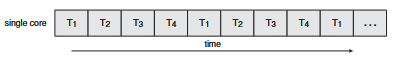
\includegraphics[width=\linewidth]{concurrency.png}
        \caption{Concurrent execution}
    \end{subfigure}
    \hspace{0.02\linewidth}
    \begin{subfigure}{0.35\linewidth}
        \centering
        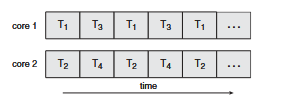
\includegraphics[width=\linewidth]{parallelism.png}
        \caption{Parallel execution}
    \end{subfigure}
    \caption{Conceptual distinction between concurrency and parallelism \cite{silberschatz2018operating}.}
    \label{fig:par_vs_conc}
\end{figure}

\subsection{Computational Models and Execution}
\paragraph{}

Computational models provide an abstract description of how tasks are executed and how
computational resources are organized during execution. These models are essential for reasoning
about the structure, scalability, and coordination of computations involving multiple activities
that progress over time.

\subsubsection{Processes}
\paragraph{}

A process represents an executing instance of a program together with its associated execution
context. This context typically includes a private address space, program code, data, and
operating system resources required for execution \cite{tanenbaum2015modern}.

Processes provide strong isolation between executing programs, as each process operates within
its own protected memory space. This isolation improves robustness and fault containment, since
errors in one process cannot directly corrupt the state of another. However, inter-process
communication generally incurs higher overhead, as it requires explicit mechanisms to exchange
data across process boundaries \cite{silberschatz2018operating}.

From an execution perspective, processes constitute units of concurrency that provide strong
isolation, at the cost of increased management and communication overhead.



\subsubsection{Threads}
\hspace{\parindent}
A thread represents a lower-level unit of execution within a process. Multiple threads within
the same process share the process address space and resources, while maintaining independent
execution contexts such as program counters and stacks \cite{tanenbaum2015modern}. This sharing
enables efficient communication and cooperation between concurrent activities, as data can be
accessed directly without inter-process communication mechanisms.

Threads can be classified according to how their management is implemented. In user-level
threading models, thread creation, scheduling, and synchronization are handled by runtime systems
operating entirely in user space. As depicted in Fig.~\ref{fig:user_kernel_threads}(a), the kernel
is unaware of individual threads and schedules only processes, while thread tables and scheduling
decisions are maintained by the runtime environment. This approach enables fast thread
management but limits the ability to exploit multiple processors transparently
\cite{silberschatz2018operating}.

In contrast, kernel-level threads, shown in Fig.~\ref{fig:user_kernel_threads}(b), are
managed directly by the operating system kernel. In this model, the kernel maintains thread
tables and schedules threads independently, allowing threads belonging to the same process to be
distributed across multiple processing units. While this enables true parallel execution on
multi-core systems, it also introduces higher management overhead due to kernel involvement
\cite{arpaci2018operating}.


\begin{figure}[H]
    \centering
    \begin{subfigure}{0.4\linewidth}
        \centering
        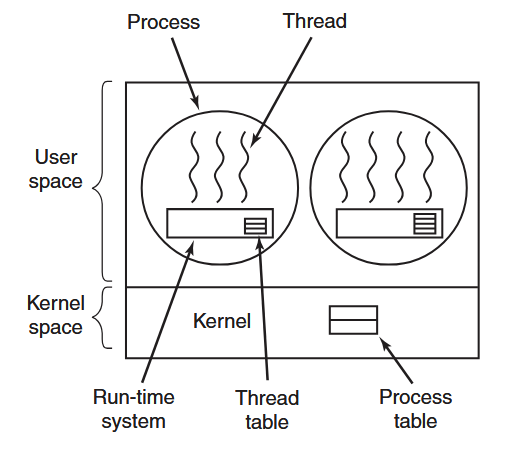
\includegraphics[width=\linewidth]{userthreads.png}
        \caption{User-level threading model}
    \end{subfigure}
    \hspace{0.02\linewidth}
    \begin{subfigure}{0.36\linewidth}
        \centering
        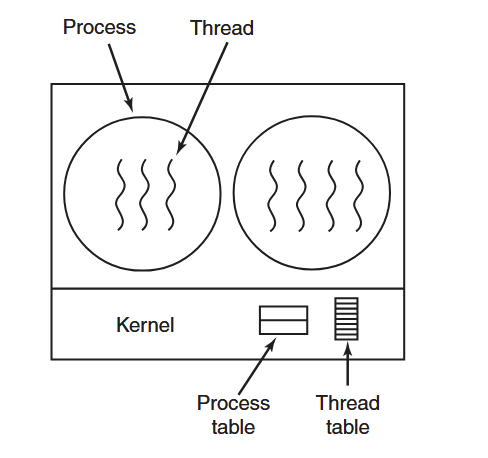
\includegraphics[width=\linewidth]{kernelthreads.png}
        \caption{Kernel-level threading model}
    \end{subfigure}
    \caption{Conceptual comparison between user-level and kernel-level thread management \cite{tanenbaum2015modern}.}
    \label{fig:user_kernel_threads}
\end{figure}

In both models, threads within a process typically share memory and other resources, adopting a
shared-memory execution model. While this model supports efficient cooperation, it also requires
careful coordination to ensure correct access to shared data. The mechanisms used to address
these challenges are discussed in the following subsection.



\subsection{Synchronization and Shared Resource Access}
\hspace{\parindent}
In concurrent execution models, multiple threads or tasks may access shared resources during
their execution. While shared access enables cooperation and efficient communication, it also
introduces challenges related to correctness, as uncontrolled interactions may lead to
inconsistent or unintended system states.

\subsubsection{Race Conditions}
\paragraph{}

In concurrent execution models, incorrect synchronization may result in race
conditions, where the behavior of a computation depends on the timing of concurrent executions. When multiple threads access shared
resources without proper coordination, the final system state may vary across different
execution schedules, even when the same operations are performed \cite{arpaci2018operating}.

Race conditions are particularly difficult to detect and reason about, as they often arise
only under specific execution orders of concurrent tasks.


\subsubsection{Critical Sections}
\paragraph{}

To prevent race conditions, concurrent systems identify regions of execution that access shared
resources as critical sections. A critical section denotes a portion of code in which a
shared resource is accessed or modified and whose execution must be mutually exclusive.

Correct concurrent execution requires that critical sections operating on the same shared
resource are not executed simultaneously by multiple threads, thereby ensuring consistency of
the shared state \cite{tanenbaum2015modern}.


\subsubsection{Mutexes}
\paragraph{}

Mutual exclusion mechanisms, commonly referred to as mutexes, provide a concrete means
to enforce exclusive access to critical sections. A mutex ensures that at most one thread may
enter a given critical section at any time.

By serializing access to shared resources, mutexes prevent concurrent modifications that could
otherwise result in inconsistent system states. This behavior is illustrated in Fig.~\ref{fig:critical}, where one process is blocked while another executes a critical section.


\begin{figure}[H]
    \centering
    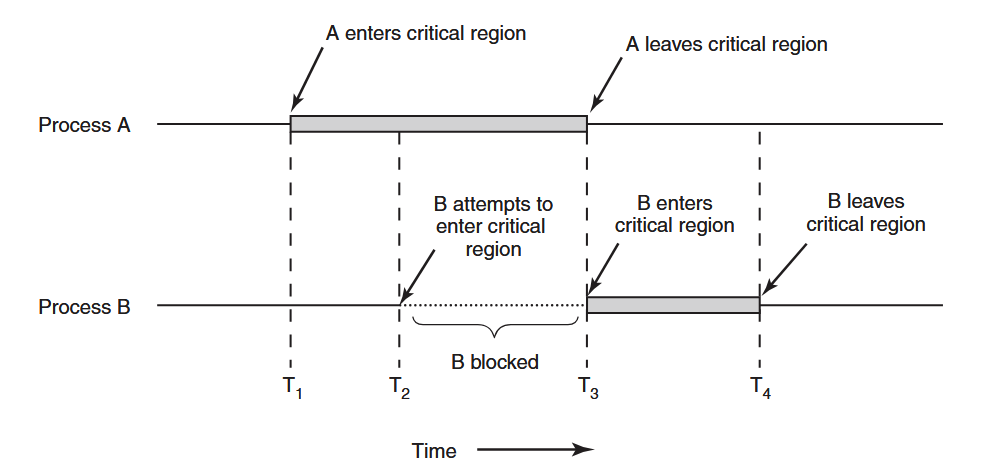
\includegraphics[width=0.8\linewidth]{critical_region.png}
    \caption{Illustration of mutual exclusion in a critical section \cite{tanenbaum2015modern}.}
    \label{fig:critical}
\end{figure}

\subsubsection{Semaphores}
\paragraph{}

Semaphores provide a general synchronization for controlling access to shared resources
and enforcing ordering constraints between concurrent tasks. Unlike mutexes, which are primarily
intended to enforce exclusive access, semaphores support more flexible coordination patterns
\cite{dijkstra1968cooperating}.

According to Arpaci-Dusseau \cite{arpaci2018operating}, semaphores are commonly
classified into two types:
\begin{itemize}
    \item \textbf{Binary semaphores}, whose value is restricted to zero or one, and which can be
    used to enforce mutual exclusion in a manner similar to mutexes, though without ownership
    constraints;
\item \textbf{Counting semaphores}, which take non-negative integer values and are used to
manage access to a finite number of identical resources. The semaphore value represents the
number of currently available resource instances and is decremented each time a resource is
allocated to a process or thread.

\end{itemize}


\subsubsection{Deadlocks}
\paragraph{}

Another fundamental challenge in concurrent systems is deadlock, a state in which a set
of threads becomes permanently blocked because each thread is waiting for resources held by
others. Deadlocks arise from circular waiting dependencies and result in a loss of system
progress, requiring careful design and coordination to avoid
\cite{silberschatz2018operating}.





\section{Summary}
\paragraph{}
This chapter introduced the main background concepts required to support the work developed in this dissertation. First, the MAPF problem was formally defined as the computation of conflict-free trajectories for multiple agents moving in a shared environment, highlighting the role of time, agent interactions, and global optimization criteria. The chapter then discussed how MAPF problems can be represented using discrete environment models, with particular emphasis on grid-based and graph-based abstractions.

Classical graph search methods were also reviewed, since they provide the basis for individual path computation in many multi-agent planning approaches. In particular, Dijkstra's algorithm and A* were introduced as fundamental shortest-path methods, together with their main properties and computational complexity.

The chapter further presented basic machine learning concepts relevant to the proposed heuristic analysis. Clustering methods, namely K-means and DBSCAN, were introduced as tools for characterizing the spatial distribution of robots, while linear regression was presented as an exploratory model for empirical runtime analysis. Finally, concepts from parallel and concurrent computing were discussed, including parallelism, concurrency, processes, threads, synchronization mechanisms, race conditions, critical sections, mutexes, semaphores, and deadlocks.

Overall, these topics establish the theoretical and technical foundation for the multi-robot planning methods, prioritization heuristics, runtime analysis, and parallel execution strategies discussed in the following chapters.